\chapter{Results}

Evaluation results of onset detection algorithms and automatic rhythm assessments are presented in this chapter. In the first experiment, various onset detection algorithms are evaluated on GuitarSet. CNNOnsetDetector is found to be performing best among them (Table \ref{tab:GSothers}). Three onset detection algorithms (CNNOnsetDetector, MC-OnsetDetector, Harmonic Onset Detector) are evaluated on both GuitarSet and MusicCritic dataset as explained in methods section (Tables \ref{tab:threeGS} and \ref{tab:threeMC}). Effects of tolerance window size are shown in Figures \ref{fig:wsize_gs} and \ref{fig:wsize_mc}.
\begin{table}
 \begin{center}
 \begin{tabular}{|l|l|l|l|}
  \hline
     & F-score & Precision & Recall \\
  \hline
  Complex & 0.67  & 0.87 & 0.59 \\
  Complex Phase & 0.59 & 0.78 & 0.52  \\
  Superflux & 0.59 & 0.46 & 0.92  \\
  NINOS$^2$ & 0.37 & 0.47 & 0.52  \\
  HFC & 0.65 & 0.79 & 0.60  \\
  RNNOnsetDetector & 0.68 & 0.82 & 0.65 \\
  CNNOnsetDetector & 0.83 & 0.78 & 0.90 \\
  \hline
 \end{tabular}
\end{center}
 \caption{F-score, Precision and Recall of various onset detection algorithms on GuitarSet}
 \label{tab:GSothers}
\end{table}

\begin{table}
 \begin{center}
 \begin{tabular}{|l|l|l|l|}
  \hline
  \textbf{Overall} & F-score & Precision & Recall \\
  \hline
  MC-OnsetDetector & 0.80 & 0.80 & 0.80 \\
  CNNOnsetDetector & 0.70 & 0.59 & 0.92 \\
  Harmonic Onset Detector & 0.85 & 0.86 & 0.84 \\
  \hline
  \hline
  \textbf{Chords} &&& \\
  \hline
  MC-OnsetDetector & 0.74 & 0.74 & 0.74 \\
  CNNOnsetDetector & 0.59 & 0.46 & 0.93 \\
  Harmonic Onset Detector & 0.84 & 0.84 & 0.85 \\
  \hline
  \hline
  \textbf{Single notes} &&& \\
  \hline
  MC-OnsetDetector & 0.85 & 0.86 & 0.84 \\
  CNNOnsetDetector & 0.78 & 0.69 & 0.92 \\
  Harmonic Onset Detector & 0.85 & 0.88 & 0.84 \\
  \hline
 \end{tabular}
\end{center}
 \caption{Performances of three onset detection algorithms on MusicCritic dataset}
 \label{tab:threeMC}
\end{table} 

\begin{table}
 \begin{center}
 \begin{tabular}{|l|l|l|l|}
  \hline
   \textbf{Overall} & F-score & Precision & Recall \\
  \hline
  MC-OnsetDetector & 0.71 & 0.95 & 0.59 \\
  CNNOnsetDetector & 0.84 & 0.78 & 0.92 \\
  Harmonic Onset Detector & 0.84 & 0.89 & 0.81 \\
  \hline
  \hline
  \textbf{Chords} &&& \\
  \hline
  MC-OnsetDetector & 0.69 & 0.95 & 0.56 \\
  CNNOnsetDetector & 0.82 & 0.78 & 0.88 \\
  Harmonic Onset Detector & 0.81 & 0.91 & 0.76 \\
  \hline
  \hline
  \textbf{Single notes} &&& \\
  \hline
  MC-OnsetDetector & 0.73 & 0.95 & 0.60 \\
  CNNOnsetDetector & 0.86 & 0.79 & 0.95 \\
  Harmonic Onset Detector & 0.86 & 0.88 & 0.86 \\
  \hline
 \end{tabular}
\end{center}
 \caption{Performances of three onset detection algorithms on GuitarSet}
 \label{tab:threeGS}
\end{table} 

On average, Harmonic Onset Detector has the highest F-score among three algorithms (Table \ref{tab:threeMC} and \ref{tab:threeGS}). On GuitarSet (Table \ref{tab:threeGS}), CNNOnsetDetector and Harmonic Onset Detector have close F-scores in both chord and single note recordings. MC-OnsetDetector's score is found to be lowest on this dataset but it has the highest precision. On MusicCritic dataset, Harmonic Onset Detector has the highest overall score with a 0.05 margin. On single notes, however, MC-OnsetDetector and Harmonic Onset Detector are close. Precision of CNNOnsetDetector, especially on chord recordings is the main reason for its low score. Precision of CNNOnsetDetector is the lowest and its recall is the highest in every category of both datasets. On MusicCritic dataset MC-OnsetDetector performs better than CNNOnsetDetector (0.1 score difference) but on GuitarSet it is the opposite (0.13 score difference).

In GuitarSet, the size of the tolerance window does not affect the scores after 0.04 seconds (Figure \ref{fig:wsize_gs}). In MusicCritic dataset, scores increase with window size for all algorithms. The score of the MC-OnsetDetector gets closer to the score of the Harmonic Onset Detector with the increasing window size. 

\begin{figure}
    \centering
    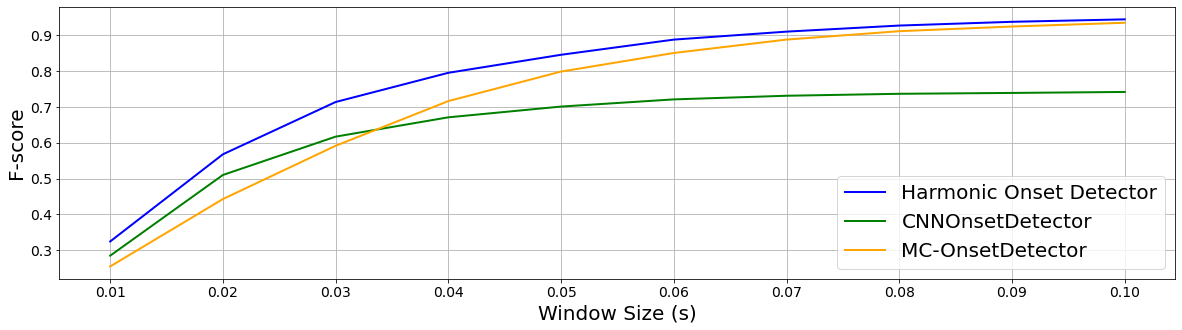
\includegraphics[width=\columnwidth]{results/mcwindowsize.png}
    \caption{F Scores of three onset detection algorithms on MusicCritic dataset w.r.t. size of tolerance window.}
    \label{fig:wsize_mc}
\end{figure}

\begin{figure}
    \centering
    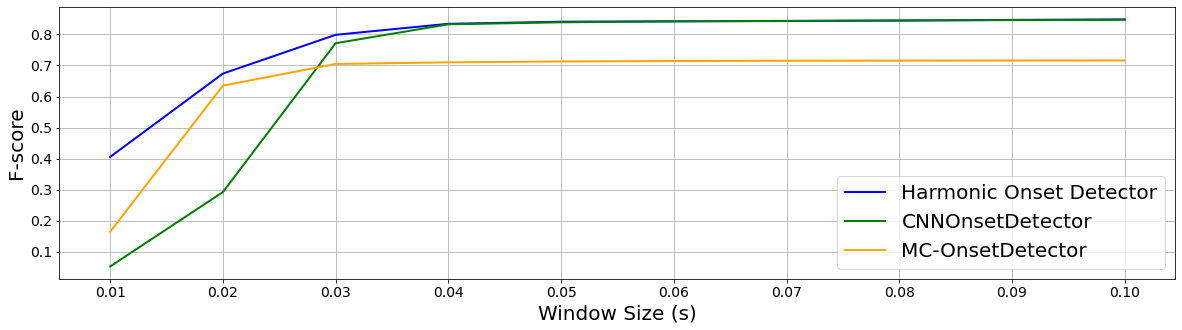
\includegraphics[width=\columnwidth]{results/gswindowsize.png}
    \caption{F Scores of three onset detection algorithms on GuitarSet data set w.r.t. size of tolerance window.}
    \label{fig:wsize_gs}
\end{figure}

\begin{table}
 \begin{center}
 \begin{tabular}{|l|l|l|l|}
  \hline
  & auto/human1 & auto/human2 & auto/humanAvg \\
  \hline
  Eremenko et al. \cite{eremenko2020performance} & 0.55 & 1.06 & 0.79\\
  MC-OnsetDetector & 0.36 & 0.76 & 0.43 \\
  CNNOnsetDetector & 0.43 & 0.98 & 0.56 \\
  Harmonic Onset Detector & 0.36 & 0.81 & 0.45 \\
  Ground truth onsets & 0.36 & 0.75 & 0.43 \\
  \hline
 \end{tabular}
\end{center}
 \caption{Mean Squared Error between grades given by human annotators and predicted grades}
 \label{tab:allassessment}
\end{table}

Onset detection results are converted to the onset difference deviations and automatic assessment experiments are conducted (Table \ref{tab:allassessment}). The first entry of the results is taken from the previous work, where MC-OnsetDetector was the algorithm used for onset detection. In the new result with the same algorithm (MC-OnsetDetector) the error is lower. The differences are the method of processing the onsets (see \ref{assessmethod}) and the recordings were trimmed when they have silences on the ends (see \ref{mc_annot}). MSE of the predictions is the lowest with MC-OnsetDetector with a 0.02 difference with Harmonic Onset Detector. MSE with the CNNOnsetDetector is higher than the other algorithms. Grade predictions did not improve when the ground truth onsets are used.  

\newpage
